\documentclass[12pt,twoside,a4paper]{article}
\usepackage{amsmath}
\usepackage{graphicx}
\usepackage{subcaption}
\usepackage[document]{ragged2e}
\graphicspath{ {../docs/} }

\begin{document}

\begin{figure}[h!]
  \centering
  \begin{subfigure}[b]{0.4\linewidth}
    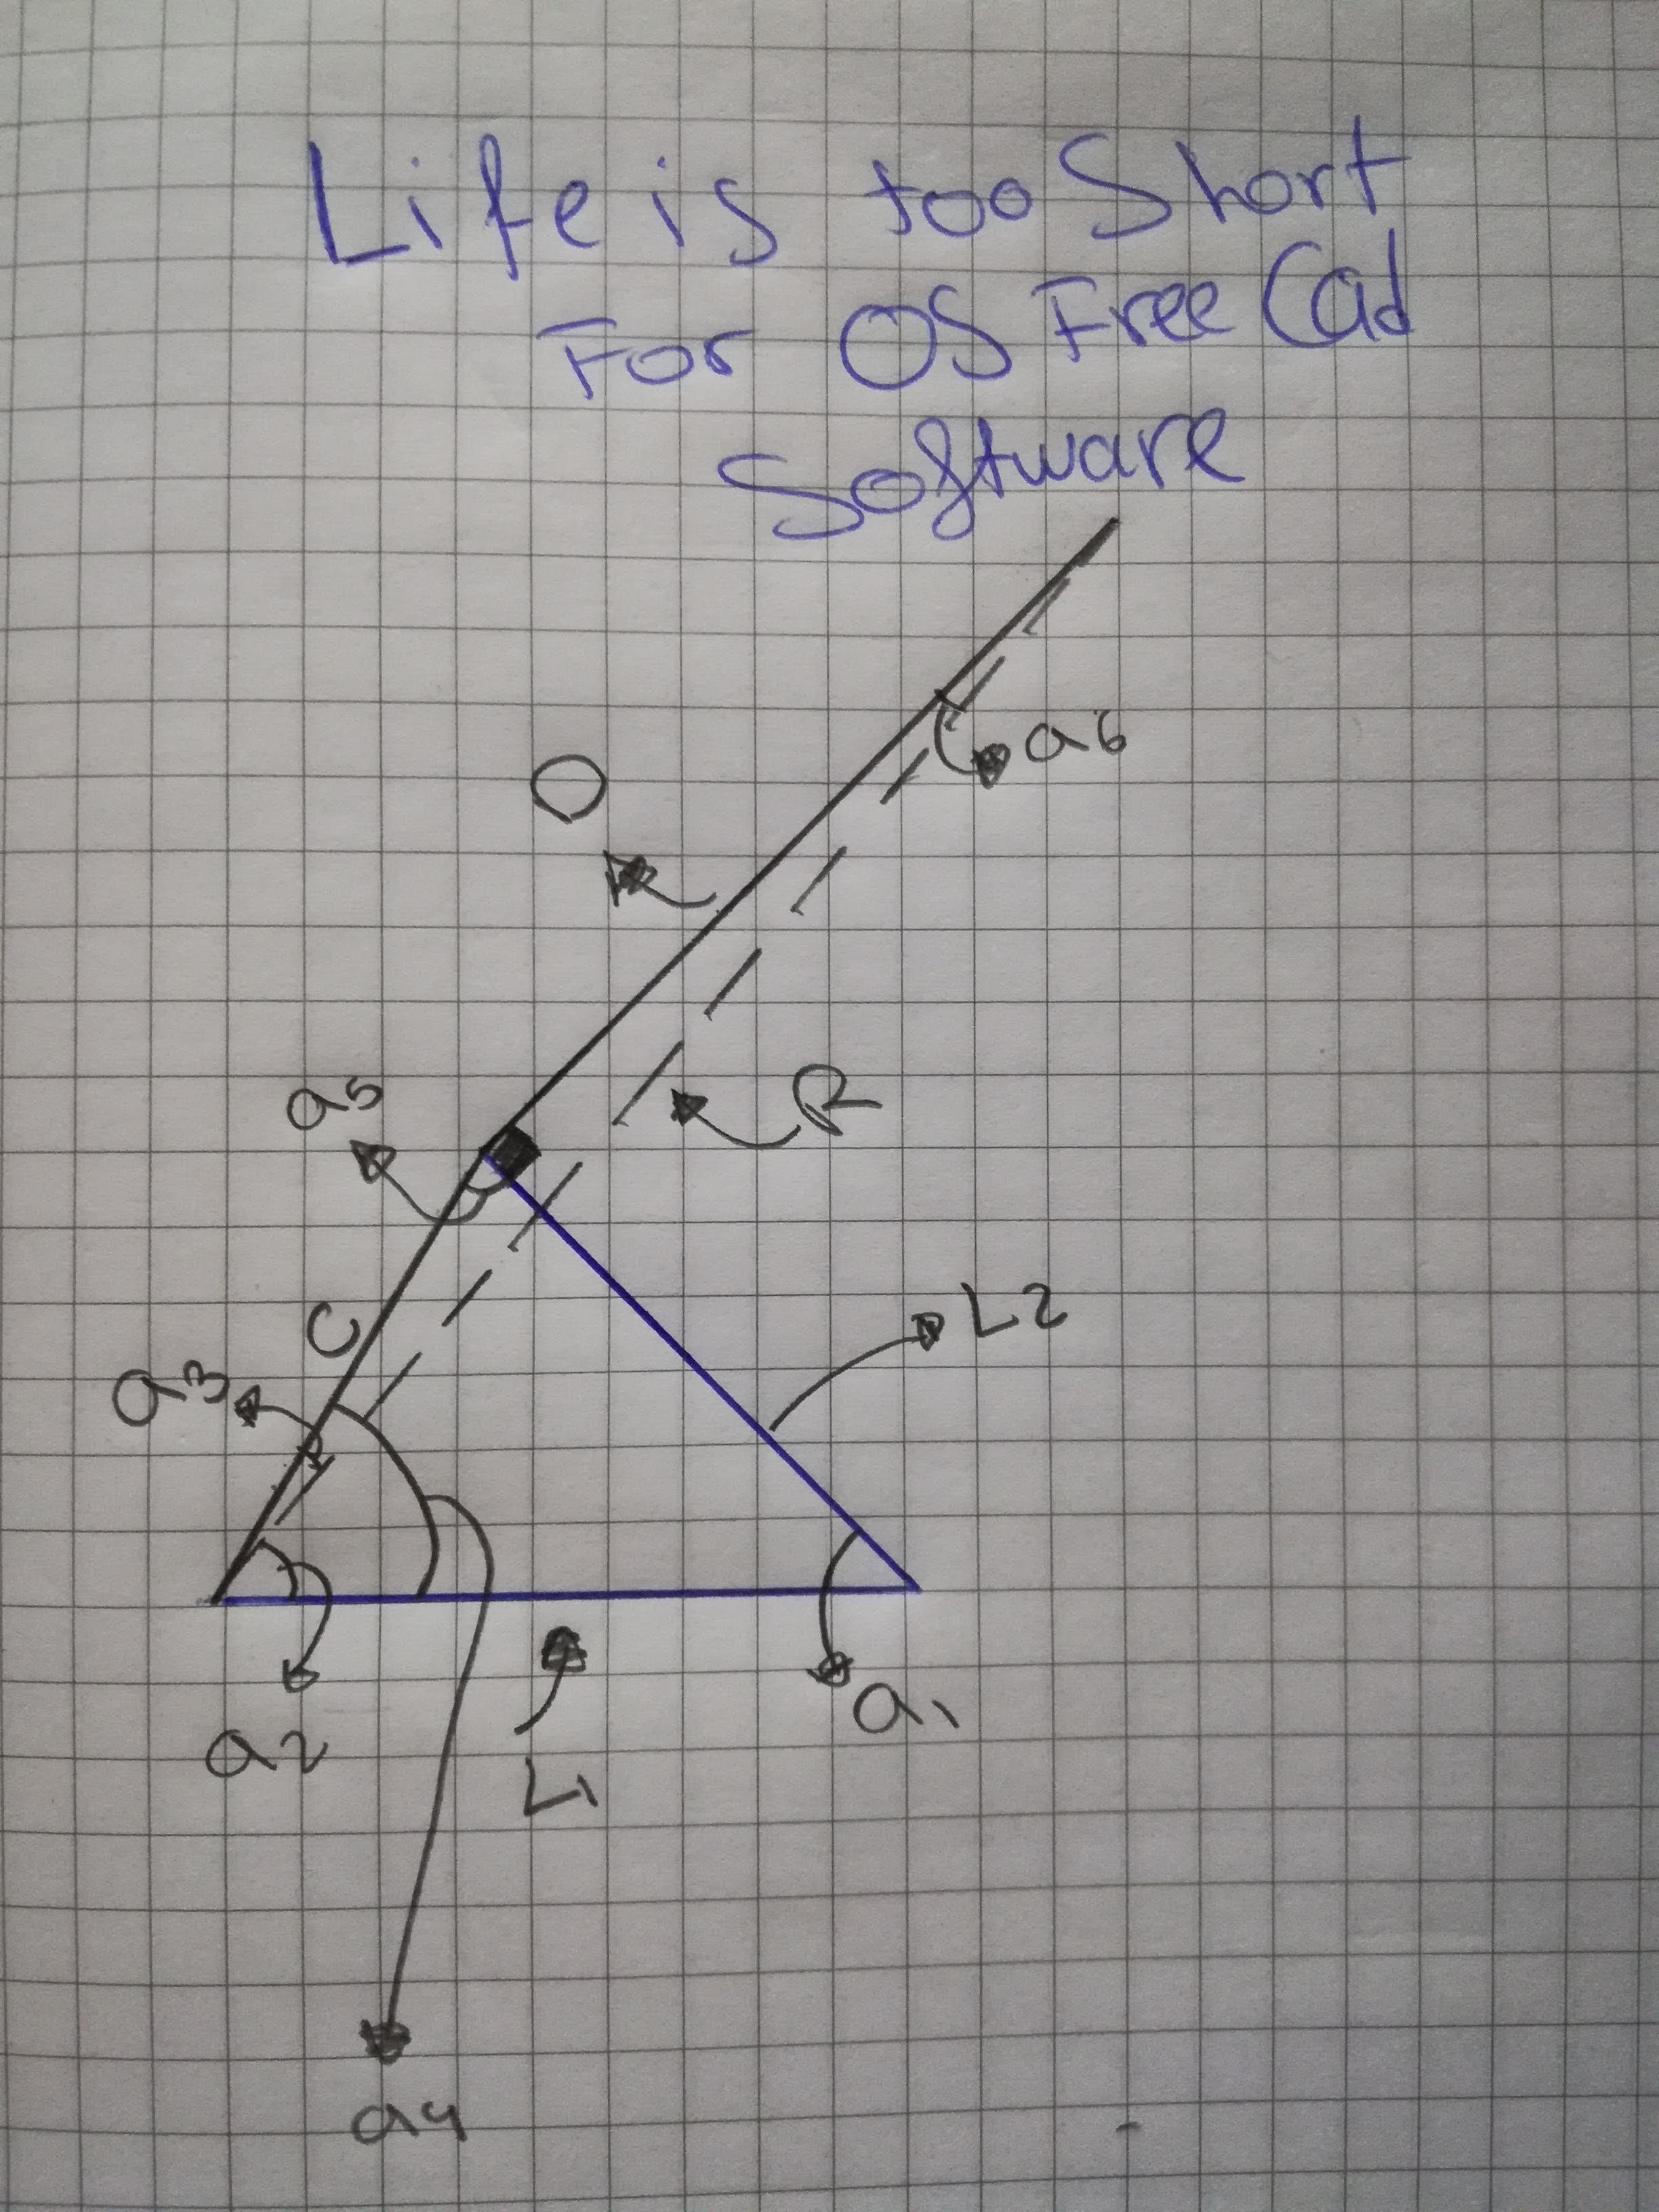
\includegraphics[width=\linewidth]{equation}
    \caption{x,y}
  \end{subfigure}
  \begin{subfigure}[b]{0.4\linewidth}
    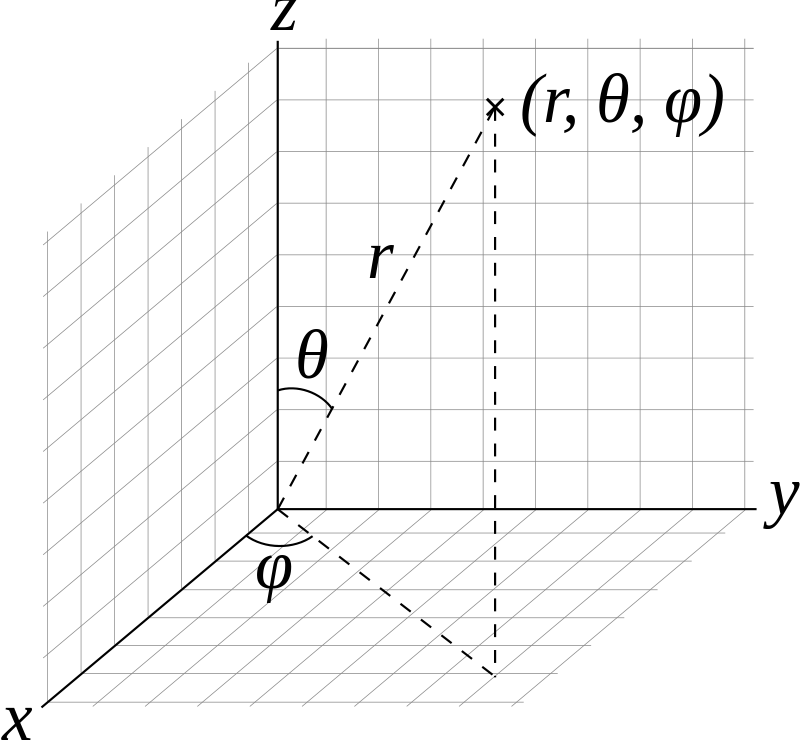
\includegraphics[width=\linewidth]{spherical}
    \caption{x,y,z}
  \end{subfigure}
  \caption{2 axis gimbal geometrical representation}
  \label{fig:coffee}
\end{figure}

\begin{flushleft}

From the servos and the sensor we get 2 angles and distance. the angle of the servo moving the sensor in the x/y plane can be used directly as the $\phi$ angle of the spherical coordinates. The radius and the $\theta$ angle will be calculated by the formulas below.
\end{flushleft}

	By applying the cosin rule on the $L_1$ $L_2$ C triangle:

	\begin{equation}
		C^2 = L_1^2 + L_2^2 -2 L_1 L_2 \cos a_1
	\end{equation}

	By applying the sine rule on the $L_1$ $L_2$ C triangle:
	
	\begin{align}
		\frac{L_1}{\sin a_5} &= \frac{C}{\sin a_1}\\
		a_5 &= \arcsin \left(\frac{L_1 . \sin a_1}{C}\right)
	\end{align}
	
	By Combining (1) and (3):
	
	\begin{equation}
		a_5 = \arcsin \left(\frac{L_1 . \sin a_1}{\sqrt{L_1^2 + L_2^2 - 2 L_1.L_2.\cos a_1}}\right)
	\end{equation}
	
	By applying the cosin rule on the R C D triangle:
	
	\begin{equation}
		R^2 = C^2 + D^2 - 2.C.D\cos(a_5+90)
	\end{equation}
	
	From the Triangle C $L_2$ $L_1$
	
	\begin{align}
		a_4 &= 180 - a_5 - a_1\\
		a_2 &= a_4 - a_3
	\end{align}
	
	From (6) and (7)
	
	\begin{equation}
		a_2 = 180 - a_5 - a_1 - a_3
	\end{equation}
	
	By applying the sine rule on the R C D triangle:
	
	\begin{align}
		\frac{R}{\sin(a_5 +90)} &= \frac{D}{\sin(a_3)} \\
		a_3 &= \arcsin \left( \frac {D.\sin(a_5+90)} {R} \right)
	\end{align}
	
	From (8) and (10)
	
	\begin{equation}
		a_2 = 180 - a_5 - a_1 - \arcsin \left( \frac {D.\sin(a_5+90)} {R} \right)
	\end{equation}
	
	From Fig 1(b)
	
	\begin{equation}
		\theta = 90 - a_2
	\end{equation}
	
	From (12) and (11)
	
	\begin{equation}
		\theta = a_5 + a_1 + \arcsin \left( \frac {D.\sin(a_5+90)} {R} \right) - 90
	\end{equation}
	
	Finally we get from (13)
	
	\begin{align}
		x &= R.\sin(\theta).\cos(\phi)\\
		y &= R.\sin(\theta).\sin(\phi)\\
		z &= R.\cos(\theta)
	\end{align}

\end{document}